% ===================================================
% CHAPITRE 26 — CONCLUSION
% Pages imprimées 275-275 — vues 278-278
% ===================================================
\chapter{Conclusion}

% --- Page imprimée 275 — vue 278
\ourouxlettrine{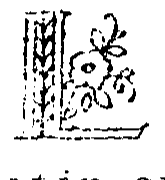
\includegraphics[height=2.6\baselineskip]{Illustrations/lettrines/conclusion.png}}{histoire d'Ouroux qui a été écrite, à votre intention, afin que vous connaissiez mieux le passé, tantôt tourmenté et laid, tantôt beau et glorieux, de ce village de France, n'est pas terminée.}

Elle continue chaque jour avec le temps qui passe. Les nouvelles pages que d'autres écriront sans doute, plus tard seront laides ou belles selon la vie des générations présentes et à venir.

Notre village porte un nom qui peut, si nous le voulons bien, résumer tout un idéal de vie. Ouroux, c'est-à-dire, comme il est expliqué au début de ce livre « lieu où l'on prie », « oratoire » doit nous inviter sans cesse à élever nos âmes vers Dieu.

Que la vue du vieux et très beau clocher fasse vivre en nos coeurs ces mêmes sentiments chrétiens qui animaient les meilleurs de nos ancêtres à qui, dans l'histoire de notre petit pays, nous devons des pages si glorieuses.

Que mes deux saints patrons d'Ouroux, Saint Antoine l'ermite et Saint Barthélemy apôtre, du haut de leur gloire céleste, veuillent bien maintenir dans le coeur de tous les habitants d'Ouroux cet idéal chrétien qui les poussera, sur cette terre, à accomplir belles et nobles choses et qui les conduira tous, un jour, auprès de ces illustres protecteurs à une vie meilleure.

J.A.
